
%-------------------------------------------------------------------------
\begin{document}

\maketitle

%-------------------------------------------------------------------------
\section{Introduction}
\label{sec:introduction}
Interactive visualization of large-scale volumetric data, produced by
simulations, astronomical instruments and high-resolution sensors, 
allows research scientists to explore scientific data, validate
hypotheses and discover new knowledge~\cite{keim2013big}. 
However, the increasing data resolution in current high-performance
computing (HPC) simulations can easily surpass the capabilities of
host systems, making interactive visualization of such data challenging. 
First, loading the full-resolution data into main memory is impractical
due to memory limitations. Second, for large datasets, the IO latency incurred by the data 
loading process is prohibitive in the existing volume renderer,
even if all the data fits into memory.
The long IO waiting time for large dataset degrades the user experience.
Therefore, research on novel techniques for
data visualization, processing, storage and IO that scale to 
extreme-scale data is required to transcend the limitations
of current hardware~\cite{beyer2014survey}.

\begin{figure*}[h]
  \centering
    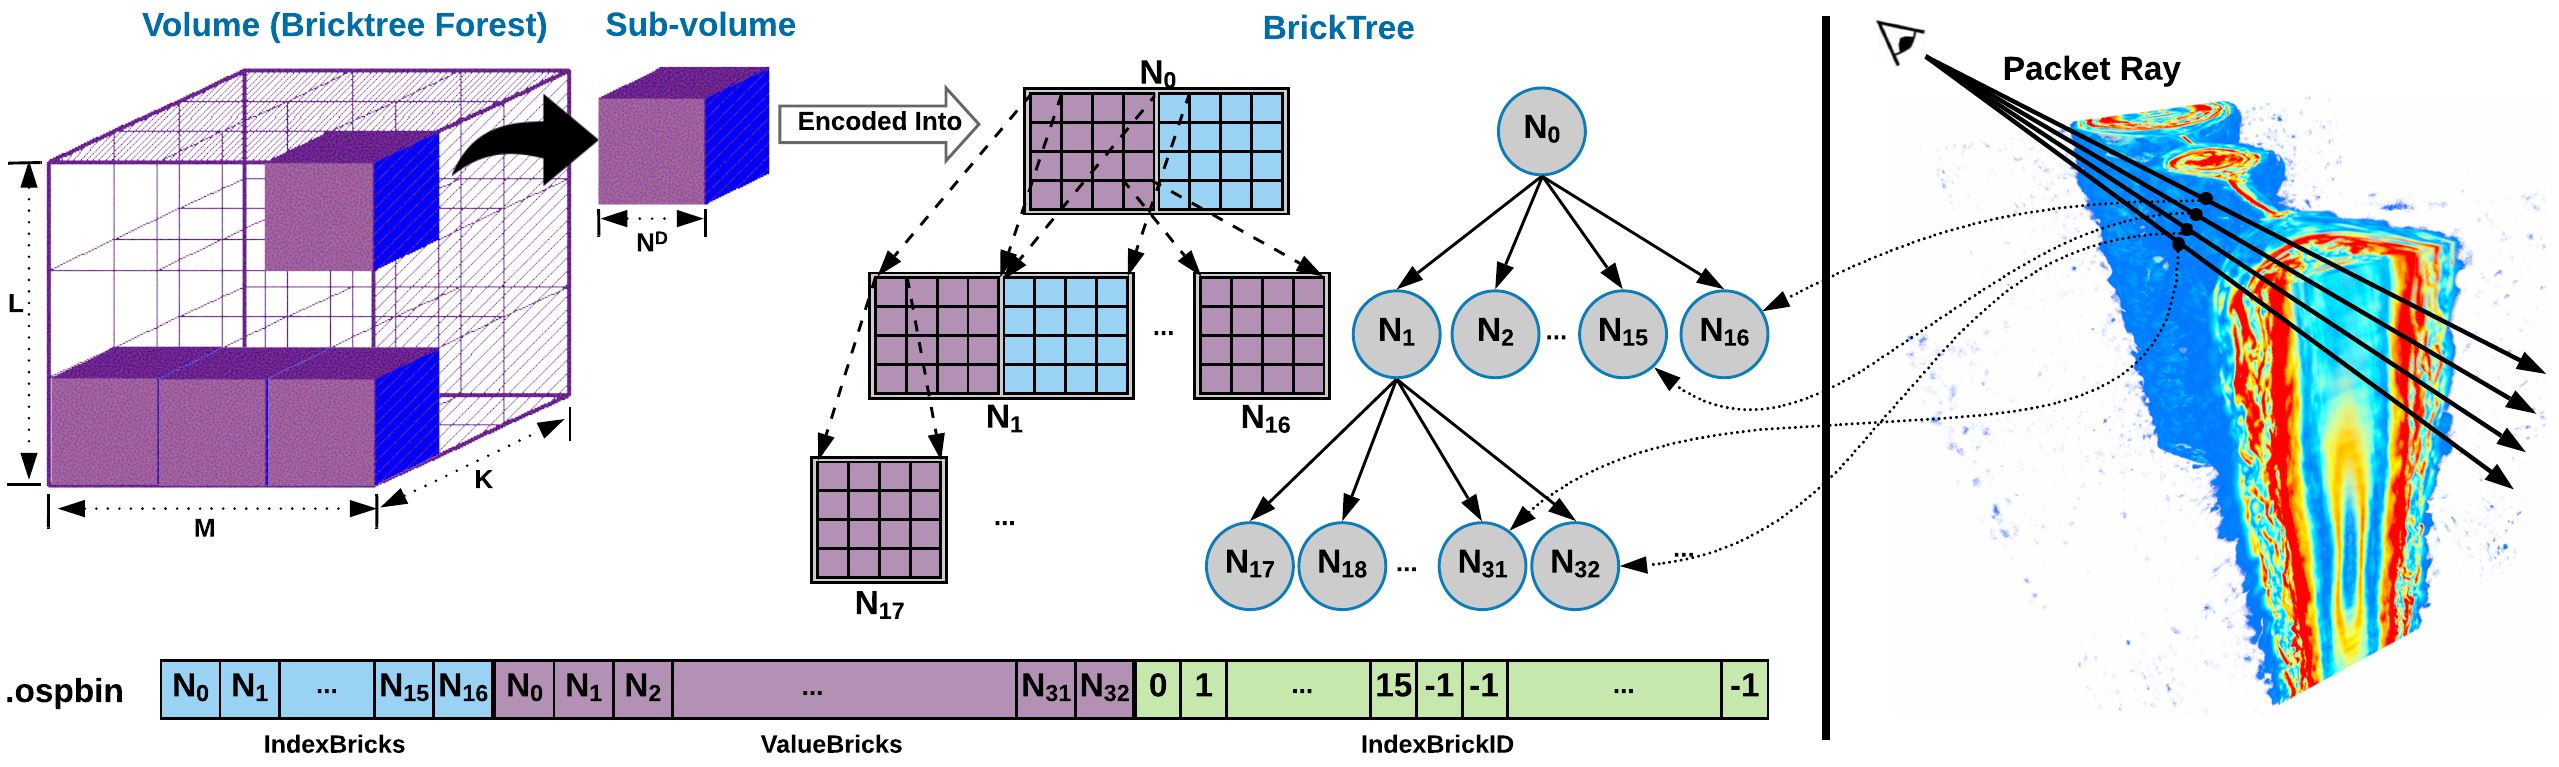
\includegraphics[width=0.99\textwidth]{BricktreeLayout}
	\caption{\label{fig:bricktree_layout}An illustration of the layout of the bricktree structure. Each brick is represented with a valuebrick (colored in purple), an indexBrickID and an optional indexbrick (colored in light blue). The indexBrickID stores the index of the indexbrick if a node has one. Otherwise, -1 is stored. Both valuebricks and indexbricks contain $N^3$ cells. 
Each cell encodes a float value in a valuebrick or an int32 reference in an indexbrick.}
    %\vspace{-1em}
\end{figure*}


Current solutions for scalable volume data visualization mostly employ GPU architecture
since it has been shown to be effective for interactive visualization. 
Prior studies~\cite{crassin2009gigavoxels,engel2011cera,hadwiger2008interactive} 
have applied out-of-core approaches, level-of-detail (LOD) techniques,
progressive rendering and data compression schemes to overcome GPU memory limitations. 
However, these approaches inevitably employ extra data structures (e.g., page tables)
and incur frequent CPU-GPU communication to refine the visible data, which hampers the interactivity. Some studies also consider architectures employing CPUs since the amount 
of memory directly accessible by a CPU often dwarfs the amount of VRAM available on even
the most powerful GPUs. Previous studies have shown that an optimized CPU volume renderer 
can outperform a GPU renderer for sufficiently large volumes ~\cite{smelyanskiy2009,knoll2011full,wald2017ospray}. However, several studies~\cite{childs2006scalable,peterka2008parallel,howison2012hybrid}
have focused on distributed parallel rendering on supercomputers, but very few have addressed interactive visualization of large-scale volumes on a single workstation.



% Due to their efficient built-in texture interpolation, GPUs have been shown to be 
% effective for interactive visualization of moderate-size volume data. 
% For large-scale datasets, 
% prior studies~\cite{crassin2009gigavoxels,engel2011cera,hadwiger2008interactive} 
% have applied out-of-core approaches, level-of-detail (LOD) techniques and
% progressive rendering to overcome GPU memory limitations. 
% However, these approaches inevitably employ extra data structures (e.g., \textcolor{blue}{page tables})
% and incur frequent CPU-GPU communication to perform visibility calculations
% and data refinement. 


% Furthermore, most of these approaches are project-specific and have not been 
% integrated into general-purpose visualization frameworks, and are thus not widely used. 

% Multi-core CPUs are a desirable platform
% for large-scale volume rendering for many reasons~\cite{knoll2011full}. The amount of
% memory directly accessible by a CPU often dwarfs the amount of VRAM
% available on even the most powerful GPUs. Previous studies have shown that an
% optimized CPU volume renderer can outperform a GPU renderer
% for sufficiently large volumes ~\cite{knoll2011full,smelyanskiy2009}.
% For purely CPU-based large-scale volume rendering systems, much 
% research~\cite{childs2006scalable,peterka2008parallel,howison2012hybrid}
% has been done on distributed parallel rendering on supercomputers. 
% However, very few previous papers have focused on interactive visualization of
% large-scale volumes on a single workstation. Furthermore, the 
% aforementioned general-purpose frameworks struggle to
% perform well on large-scale data. 

In this work, we present an interactive visualization solution for large-scale
volumes on multi-core CPU architectures. Our solution allows users to get an overview of the large
data in seconds rather than minutes or hours using existing visualization frameworks. 
We build our approach on a hierarchical data structure -- \textit{Bricktree} -- that allows
for a hierarchical representation of the volume. During the rendering, we stream the
necessary data on demand with separate threads and employ ray-guided progressive
rendering for data refinement. As an extension of the OSPRay ray tracing 
framework, which already contains various techniques for visualizing scientific data \cite{wald2017ospray,wang2018cpu}, we build a bricktree
module along with an efficient hierarchy generation tool to support large-scale data
visualization on multi-core workstations. Given that OSPRay has been integrated into
Paraview and VisIt, our module is ready to be integrated into general-purpose
visualization frameworks. Specifically, our contributions in this paper are:

\begin{itemize}
\item An interactive visualization solution for large-scale volume
visualization, which decouples the data loading and rendering process 
on multi-core architectures and dramatically reduces the amount of time the user has to
wait before being able to explore the data. 
\item The Bricktree, an efficient and low-overhead hierarchical structure that
allows for encoding a large volume into a multi-resolution representation.
We also evaluate the structure with several choices of parameters. 
\item An OSPRay module for large data visualization
and a parallel hierarchy generation tool that are ready to be 
"dropped into" a general-purpose visualization pipeline.  
\end{itemize}



%-------------------------------------------------------------------------
\section{Previous Work}

Although widely used for visualization of 3D scalar fields, volume rendering
remains a computation, memory and I/O-intensive task~\cite{wu2018visit}. 
Several studies have focused on improving the rendering performance by
introducing efficient packet BVH traversal~\cite{knoll2011full,wald2017ospray}, 
empty space skipping~\cite{hadwiger2018sparseleap} and
early ray termination~\cite{levoy1990efficient,kruger2003acceleration}.
Although efficient for visualizing moderate-size volumes on consumer desktops, 
these methods struggle to scale to petascale or exascale datasets since they assume that the entire volume is present in memory. 
% these methods 
% assume that the entire volume is present in memory and struggle to scale
% to petascale or exascale datasets.
Previous work on large-scale volume rendering
can be categorized as: 

1) Parallel/distributed rendering on distributed memory systems. These approaches
parallelize data processing over many nodes~\cite{childs2010extreme}. Research
has demonstrated strong scalability on both CPU and GPU clusters~\cite{childs2006scalable,
howison2012hybrid,peterka2008parallel,eilemann2009equalizer,fogal2010large,beyer2011distributed}. 
For example, Howison et al.~\cite{howison2012hybrid} demonstrated that MPI-hybrid
parallelism achieves a sublinear raycasting speed-up and is more efficient in terms of
overall speed and memory than the MPI-only parallelism.
However, previous work~\cite{wu2018visit} has found that the main
performance bottleneck of distributed visualization lies in final image compositing
rather than in the volume rendering process.

2) Visualization of large-scale volumes on a stand-alone workstation.
Much effort has been devoted to the implementation of GPU renderers
due to the great hardware interpolation capabilities\cite{feng2015parallel}.
Beyer et al.~\cite{beyer2014survey} conducted a detailed survey on this topic. Most prior work focuses on overcoming the GPU's
memory limitation and tackling this issue by loading only the visible
part of the volume into GPU memory~\cite{li2003empty}. 
The GigaVoxels system~\cite{crassin2007interactive,crassin2009gigavoxels}, the first to employ this idea, determines the visibility of
small blocks ``on the fly''.  
Although capable of rendering several billion voxels in real-time,
it mainly focuses on entertainment applications and targets sparse volume datasets.
CERA-TVR~\cite{engel2011cera} then extended the GigaVoxel paper, 
targeting scientific visualization user cases.
In contrast to GigaVoxel, CERA-TVR is capable of rendering dense volumes
and can progressively refine parts of a framebuffer if the size of the visible
data exceeds the size of the brick pool.
Hadwiger et al.~\cite{hadwiger2012interactive} proposed a virtual memory scheme
that avoids explicit tree traversal and supports interactive visualization and 
streaming of petascale 2D image data. However, this approach exhibits
IO latency during 3D block construction due to cache misses and requires that all
visible data fit into cache. All these approaches inevitably require
heavy CPU-GPU communication, which significantly impacts interactivity. 


In the context of the CPU-based renderers, very little research has focused
on large-scale volume rendering on multi-core workstations.
As a state-of-art CPU ray-tracing framework for scientific visualization,
OSPRay works well for interactive visualization of moderate-size volume data
and can potentially be extended to large-scale data.
Wu et al.~\cite{wu2018visit} proposed the VisIt-OSPRay system, which can scale to
large-scale datasets. To achieve interactive visualization, they integrated OSPRay
into VisIt as a backend visualization toolkit and coupled it with PIDX (parallel IO 
library)~\cite{kumar2011pidx} for scalable IO. 
This study achieved interactive visualization, but it took more than 30 minutes to load the DNS 
dataset into memory with 64 processors on Stampede2.
%(a supercomputer at the Texas Advanced Computing Center (TACC)). 

To address these challenges, we decompose large volumes into a hierarchical 
representation, with each node representing a small cubic brick. Within the rendering pipeline,
we leverage ray-guided streaming and progressive rendering to reduce IO latency. 



%-------------------------------------------------------------------------
\section{Bricktrees}

\feng{Adaptive space subdivision and hierarchical data representation are
key to interactive visualization of large-scale volumetric datasets\cite{crassin2009gigavoxels}.
These techniques enable us to load and update the working-set on-demand to address IO latency
and memory limitations. As a popular hierarchical data structure for 3D space subdivision,
the octree has been well studied for direct volume rendering\cite{gobbetti2008single}.
Hierarchical grids feature a theoretically optimal number of traversal steps,
and thus have been overtaken as general-purpose ray tracing acceleration structures
\cite{knoll2006interactive}. Lefebvre et al.\cite{lefebvre2005octree} proposed
the $N^3$-tree, which is capable of dividing each edge by an arbitrary number N
rather than 2. $N^3$-tree was later used in the GigaVoxel system
\cite{crassin2009gigavoxels}. Other structures, such as 
kd-trees, were also used in isosurface rendering with the trend of coherent
ray tracing\cite{wald2001interactive,procopiuc2003bkd,wald2005faster}. 
}

\begin{figure}[h]
  \centering
  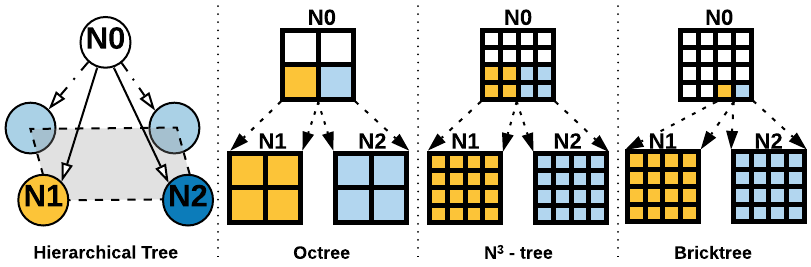
\includegraphics[width=\columnwidth]{tree_comparision}
  \caption{\label{fig:tree_comparision}Comparision of an octree, an $N^3$-tree and a bricktree(2D representation).
  An octree has a branching factor of 8 and allows for dividing a node by 8; A $N^3$-tree has a branching factor
  of 8 and allows for dividing a node by $N^3$; A bricktree has a branching factor of $N^3$ and allows for
  dividing a node by $N^3$.}
    %\vspace{-1em}
\end{figure}
%Adaptive space subdivision and hierarchical data representation are key to
%interactive visualization of massive volumetric datasets\cite{crassin2009gigavoxels}. 
%For large data visualization, these techniques enable us to load and update
%the working-set on-demand to address memory limitations and IO latency. 
%As a regular hierarchical data structure, the octree has been
%well studied for volume rendering\cite{gobbetti2008single}.
%Hierarchical grids feature a theoretically optimal number of traversal steps,
%and thus have been overtaken as general-purpose ray tracing acceleration structures
%\cite{knoll2006interactive}. Lefebvre et al.\cite{lefebvre2005octree} proposed
%the $N^3$-tree, which is capable of dividing each edge by an arbitrary number N
%rather than 2. $N^3$-tree was later used in the GigaVoxel system
%\cite{crassin2009gigavoxels}. Other structures, such as 
%kd-trees, were also used in isosurface rendering with the trend of coherent
%ray tracing\cite{wald2001interactive,procopiuc2003bkd,wald2005faster}. 

\feng{
In this work, we define a hierarchical data structure --``bricktree''-- which allows
us to represent a structured volume in a hierarchical, multiresolution and compressed
way (as shown in \Cref{fig:bricktree_layout}).
Rather than encoding the large volume into a single deep bricktree, our design
tiles the volume into a ``bricktree forest'' which consists of a list of bricktrees.
This design is not only conducive to parallel tree traversal on multi-core CPU architectures,
but also avoid encoding a large empty space when the structured volume is a cuboid ($M \neq L \neq K $).
A bricktree is a generalization of an octree when we subdivide a node by an arbitrary number
$N^3$ rather than by 8. Furthermore, a bricktree is similar to an $N^3$-tree but with an arbitrary
branching factor $N^3$ rather than by 8 (as shown in \Cref{fig:tree_comparision}). 
}

%In this work, we define the ``bricktree'' data structure, which allows us to
%represent a structured volume in a hierarchical, multi-resolution
%and possibly compressed way (as shown in \Cref{fig:bricktree_layout}).
%A single bricktree is similar to an $N^3$-tree but with a larger branching factor. 
%Rather than encode the large volume into a single deep bricktree, our design
%tiles the volume into a bricktree forest. This design is conducive to parallel tree traversal on multi-core CPU architectures.

%----------------------------------
\subsection{Data Layout}
\label{sec:bricktree_layout}

\feng{
In \Cref{fig:bricktree_layout}, the structured volume with dimension of $M\times L \times K$ is 
organized into a bricktree forest. Each bricktree, which is specified through a brick size (N), a data
type (T) and a tree depth (D), represents a range of $N^D \times N^D \times N^D$ voxels in the volume.
In particular, a given bricktree consists of a series of unidirectional linked nodes (bricks).
Bricks, therefore, form a natual hierarchy of branching factore $N^3$.
In our design, a brick represents $N^3$ cells with each could store a data value or a reference to a 
child brick. We name a brick whose cell stores the data value as a valuebrick and the reference as an 
indexbrick. In the hierarchy, a brick is represented with a valuebrick, an optional indexbrick and
an indexbrickID to indicate the corresponding indexbrick. Seen in \Cref{fig:bricktree_layout}, an
inner brick (e.g. $N_0$) is along with a valuebrick, an indexbrick and an indexbrickID.
Whereas a leaf node (e.g. $N_{16}$) is represented with a valuebrick and an indexbrickID
which is set to invalid (-1).
}

\feng{
Each cell in a valuebrick corresponds to a region of voxels in the logical volume space.
For a leaf brick, the cell exactly corresponds to one logical
volume voxel, and the cell's value equals the value of the corresponding voxel.
The cells of an inner brick typically refer to voxels that the child brick
corresponds to. Accordingly, the cell's value equals the average of the
voxel's value. 
}

\feng{
Each cell in an indexbrick can -- but is not required to -- refer to a child brick with a child index.
The child indices are encoded through two level of indirection: first, if a brick don't have an indexbrick
or the indexbrickID is marked as invalid, then none of the brick's cells have children; If the brick have
an indexbrick, we further check the child index that is stored in the indexbrick's cell. The child index 
indicates the location of the child brick. A given cell does not have children when its corresponding
child index is marked as invalid. 
}

%Each bricktree is specified through a brick size N, a data
%type T and a tree depth of D. A full bricktree of depth D is called a
%``block'', which represents a range of $N^D \times N^D \times N^D$ cells.
%If one block is not sufficient to represent the whole input
%volume (i.e., $M,L,K > N^D$), we generate as many blocks as
%required to tile the entire volume. A bricktree ``forest'' is composed of all the blocks.
%In particular, a given bricktree consists of a series of ``bricks'' that
%usually represent $N^3$ cells. Each cell contains one value and can
%refer to a child brick. Bricks, therefore, form a natural hierarchy of
%branching factor $N \times N \times N$.

%Each cell in a brick corresponds to a region of voxels in the logical volume 
%space. For a leaf brick, the cell exactly corresponds to one logical
%volume voxel, and the cell's value equals the value of the corresponding voxel.
%The cells of an inner brick typically refer to voxels that the child brick
%corresponds to. Accordingly, the cell's value equals the average of the
%voxel's value. 

%In our design, each cell can -- but is not required to -- refer to a child brick. 
%A brick's child indices are encoded through two levels of indirection: first, each
%brick can (but does not have to) have an index brick. 
%If it does not have an index brick or the index brick is marked as invalid,
%then none of the brick's cells have children. 
%If the brick does have an index brick, we further check the child index
%that is stored in the index brick's cell. A given cell does not have children 
%when its corresponding child index is marked as invalid. 

In memory, each $BrickTree<N,T>$ is represented as three linear arrays:
\begin{enumerate}
\item One linear array of ``valuebricks'', where each valuebrick contains
$N \times N \times N$ values of type T.
\item One linear array of int32 ``indexbrickIDs'', with exactly one such
int32 per valuebrick. If a given valuebrick's indexbrickID is
invalid, it does not refer to an indexbrick and thus has no children;
otherwise, this ID refers to an indexbrick in the indexbrick array.
\item One linear array of ``indexbricks``, where each indexbrick contains
$N \times N \times N$ int32 indices. Each such index can be invalid (meaning the
corresponding cell does not have a child); 
if the index is greater than or equal to 0, it refers to a brick in the valuebrick array.
% (which in turn can have childrenreferred to it's index brick ID, etc).
\end{enumerate}

On a file system, the whole volume is represented by one ``\textit{.osp}'' file
that contains meta-data ($N,T, (M,L,K)$ of input volume, etc). 
Each bricktree is stored in two files: 1) an ``\textit{.osp}'' file that
gives high-level information ($N, T, D$, etc.) in \textit{XML} form; 
2) an ``\textit{.ospbin}'' file that contains the three arrays in binary form.


%----------------------------------
\subsection{Bricktree Overhead}
Due to the specific layout, our bricktree is easy to index and the overhead is low. 
Given a bricktree with a brick size of 4, a data type of float and a depth of 4 ($bricktree<4,float>$), a certain number of $4^3$ valuebricks and $4^3$ indexbricks will be generated when building the tree.
In practice, leaf valuebricks have zero overhead, since each costs 
exactly 256 bytes for 64 float-typed cells. The only overhead lies in the 
indexbricks and inner valuebricks. However, few of these bricks exist relative
to the number of leaf bricks (see  \Cref{fig:loadbylevel}).

\feng{
Let us take a close look at indexbricks. In an ideal case where many of the inner 
nodes all point to the leaf valuebrick, we store only about one int (4~byte)
for a complete leaf valuebrick. Hence, 4~bytes are used to index 256 ``payload''
bytes for float data. A less ideal case is that some children of inner nodes are leaf
valuebrick, and other children are inner nodes. In this case, we need to store 
a valuebrick as well as an indexbrick for those children that are inner nodes. 
There will be some additional memory consumption in contrast to the ideal case.
However, the overhead most likely will be considerablely less than for an octree. 
A proof shows in \Cref{table:brick_size} that the size of a bricktree with N = 4 is much 
less than a bricktree with N = 2 which is technically an octree. 
In addition, few valuebricks are located in the upper levels of the tree. Assuming a brick
size of 4, the number of inner nodes goes down by a factor of 64 each time we go up one level
in the tree. This holds in practice - the overhead is 8.0\% on the magnetic dataset 
(see \Cref{fig:exp_threshold_2}) and the DNS dataset (see \Cref{table:brick_size}) with $N=4$. 
}

%----------------------------------
\subsection{Hierarchy Generation in Parallel}
\label{sec:hierarchy_generation}

As an offline process that is usually run in advance, the performance of reorganizing the volume
into multi-resolution bricks is mostly ignored in the volume rendering literature\cite{fogal2013analysis}. However, it becomes a significant
bottleneck for large-scale datasets. As illustrated in \cite{fogal2013analysis},
the runtime for building a hierarchical structure for RMI (8.1~GB, 
$2048 \times 2048 \times 1920$) is up to 1.5 hours in the worst case and 13 minutes in the best case. 
Petascale datasets might take hours or days. 
The virtual memory architecture of \cite{hadwiger2012interactive} alleviates this
problem by constructing the brick at runtime. However, the latency of constructing
bricks at runtime will dramatically influence the framerate, especially when the 
visible data is missing in memory. 

\feng{
The design of the bricktree forest contributes to improving the efficiency of hierarchy generation. 
It is straightforward that we can construct the bricktrees in parallel. The ``\textit{ospRawToBricks}''
tool, which employs the \textit{GNU make} command, is used to meet this end.
Normally, \textit{make} will execute only one recipe at a time.
By specifying the ``\textit{-j}'' option, it is possible to execute many recipes simultaneously.
Once parameters $N$, $T$ and $D$ are set, we first generate the index file of bricktrees
as well as a makefile, which will then be used to build each bricktree in parallel.
\Cref{alg:bricktree} shows the pseudocode of recursively constructing a bricktree. 
An evaluation of performance improvement with multiple processes is shown in
\Cref{fig:exp_buildtime}.
}


\begin{algorithm}
	\caption{The recursive function for constructing a bricktree. $N,T$ is defined as a template parameters.
	Threshold is a customized parameter for ``compression''.}\label{alg:bricktree}
	\begin{algorithmic}[1]
		\Function{BuildRec}{$avgValue, llCoord, level, levelWidth$}
			\State $cellSize \gets levelWidth / N $
			\State $brick, vRange$
			\If {levelWidth ==  N}
				\State $brick.value[i][j][k] \gets input.get(N * llCoord + offset)$
				\State $vRange.extend(brick.value[i][j][k])$
			\Else
				\State $vRange \gets BuildRec(avg,N*llCoord + offset, level+1,cellSize))$
				\State $brick.value[i][j][k] \gets (T)avg$
			\EndIf
			\State $avgValue \gets brick.ComputeWeightedAverage()$
			\If{$vRange \leq threshold$}
				\State \textit{This is a valueBrick with same value.}
				\State \textit{Kill this brick (value has been saved in parent node).}
			\Else
				\State \textit{Set this brick into the brick buffer.}
			\EndIf
			\Return $vRange$
    	\EndFunction
	\end{algorithmic}
\end{algorithm}



%One advantage of constructing a bricktree forest is that the hierarchy 
%generation process can be executed in parallel. The ``\textit{ospRawToBricks}''
%tool, which employs the \textit{GNU make} command, is used to meet this end.
%Normally, \textit{make} will execute only one recipe at a time.
%By specifying the ``\textit{-j}'' option, it is possible to execute many recipes
%simultaneously.
%Once parameters $N$, $T$ and $D$ are set, we first generate the index file of blocks
%as well as a makefile, which will then be used to build each block of the
%bricktree forest. 

\feng{
In addition, the builder also supports data format conversion and ``compression''.  
The format conversion allows us to convert an input format to an interval format, such as double to float.
The ``compression'' is automatically supported by letting the user specify a
threshold that indicates which input regions can be safely collapsed.
This process is also known as empty space skipping.
For instance, a cell will be automatically stored as a leaf 
if the cell's value range in an entire region is less than the threshold. 
The default threshold value is 0, meaning that it losslessly eliminates
equal-value regions.
}

%-------------------------------------------------------------------------
\section{Volume Integration}
In this section, we illustrate the rendering pipeline with bricktrees in a
simple case where all data have been read into memory.  
Raycasting-based volume rendering consists of marching rays through the volume with
a step size and accumulating color and opacity along the ray. With a hierarchical
structure, rays need to traverse the structure until reaching a leaf node, an inner
node with appropriate level-of-detail in current view or an unmapped node. 

% In contrast to hierarchical structures provided by current GPU-based approaches 
% \cite{crassin2009gigavoxels, hadwiger2012interactive},
% the CPU allows for greater control over these structures\cite{knoll2006interactive}.

\begin{algorithm}
	\caption{Pseudocode on sampling a given point $p$ and traversal of the bricktree structure }\label{alg:sample}
	\begin{algorithmic}[1]
		\Procedure{Bt\_Cplus\_Sample}{$p$}
        	\State $valueArray[8]\gets \textit{0}$
            \State $\textit{voxelCoord[8]} \gets \textit{Calculate 8 vertex's coordinates}$
            \While{$i < 8$}
            	\State $blockID \gets ComputeBlockID(voxelCoord[i])$
            	
                \State $bt \gets GetBrickTree(blockID)$
            	\State $valueArray[i] \gets Bt\_Cplus\_GetVoxels(bt,voxelCoord[i])$
            \EndWhile
            \State $result \gets lerp(valueArray[8])$
            \State \textbf{return} $result$
    	\EndProcedure
        \Procedure{Bt\_Cplus\_GetVoxels}{$bt, coord$}
        	\State $brickID\gets \textit{0}$\Comment{top-down traversal}
            \State $brickStack.push(brickID)$
            \While{brickStack is not empty}
            	\State $cBrickID \gets brickStack.pop()$
                \State $ibID \gets bt.brickInfo[cBrickID].indexBrickID$
            	\State $cOffset \gets ComputeOffset(coord)$
                \State $childBrickID \gets bt.indexBrick[ibID].child[cOffset]$
                \If {$childBrickID = -1$} 
                	\State \textbf{return} $bt.valueBrick[cBrickID].child[cOffset]$
                \Else
                	\State $brickStack.push(childBrickID)$
                \EndIf
            \EndWhile
    	\EndProcedure
	\end{algorithmic}
\end{algorithm}

%Now we describe bricktree traversal on the many-core CPUs. 
For a given sample point $p$ along a ray, we need to query the value of eight
neighboring voxels for interpolation. For each voxel, a tree traversal
is needed to fetch the valuebrick that the voxel belongs to. We start the bricktree
traversal from the root node. Assume that we operate on brick 1 of a 
$BrickTree<4,float>$ and want to know if its cell $(1,1,2)$ has a child.
First, we look up the brick's index brick ID ($ibID = indexBrickID[1]$).
We know that none of the cells of brick 1 have a child if the $ibID$
is invalid or less than 0. If this is the case, cell $(1,1,2)$ certainly does not have a child.
However, if $ibID \geq 0$ (e.g., $ibID = 1$ in \autoref{fig:bricktree_layout}), 
then we look at $cellChildID = IndexBrick[ibID].child[1][1][2]$. 
If this value is invalid (-1), then this particular cell of brick 1 does not have any
children. Otherwise, $valueBrick[cellChildID]$ is the child brick.

Algorithm \ref{alg:sample} describes the general sampling process. 
Trilinear interpolation of eight nodal value is used to determine the value of an 
arbitrary point $p$. $Bt\_Cplus\_GetVoxels$ traverses the bricktree and queries the 
value of a given cell. 

So far, we have obtained a sample kernel that has access to the bricktree ``forest'' and is 
implemented with C++ code. However, as a loadable module to the OSPRay ray tracing
framework, our bricktree module employs the OSPRay rendering pipeline, which is internally
built on top of Embree\cite{wald2014embree} and ISPC\cite{pharr2012ispc}. Embree is
a collection of high-performance ray tracing kernels. 
The Intel SPMD Program Compiler (ISPC) allows a number of program instances
to execute in parallel on SIMD hardware. ISPC compiles its own programming language
(a variant of C), and this ISPC code can call and be called from C/C++ application code.
In OSPRay, the sampling process maps well to the SIMD paradigm, and is thus implemented
with ISPC code. Under this condition, we can have two approaches to implement our
sampling process. 


% ISPC, which is the Intel SPMD
% Program Compiler, supports that a number of program instances execute the application
% in parallel on hardware.
% In the OSPRay rendering pipeline, the sampling process is implemented with ISPC code
% since it is independent. Under this condition, there are two approaches to implement
% our sampling process. 

% Note that we construct the bricktree forest with C/C++ code and visualize the hierarchical
% structure within the OSPRay ray tracing framework, which is internally built on top of
% Embree\cite{wald2014embree} and ISPC\cite{pharr2012ispc}.
% We fully utilize modern instruction sets on many-core CPU architectures. 
% \par
% We will now discuss several different ways to implement the sample function. 


%----------------------------------
\subsection{C/C++ Serial Implementation}

A simple but inefficient approach is a serial implementation with C/C++ code without
maintaining a copy of the bricktree structure on the ISPC side. We can easily 
implement a C/C++ version of the sample function (see \cref{alg:sample}) that has direct
access to the bricktree structure, and call it serially from the ISPC sample callback
function. The \textbf{\textit{foreach\_active}} construct is
utilized to specify a loop that iterates over the active program instances serially.
The loop executes once for each active program instance, and with only that program
instance executing. Algorithm \ref{alg:ispc_sample} depicts the process of serially calling 
the C/C++ implementation of sampling function from the ISPC code (\textit{programCount},
\textit{programIndex}, \textit{lane} are built-in variables in ISPC). 

\begin{algorithm}
	\caption{Pseudocode for serially calling the C++ version of sampling function from ISPC code. }\label{alg:ispc_sample}
	\begin{algorithmic}[1]
		\Procedure{Bt\_ISPC\_Sample}{\textbf{varying} samplePos}
        	\State \textit{\textbf{uniform} uPos[programCount]}
            \State \textit{\textbf{uniform} uValue[programCount]}
            \State $uPos[programIndex] \gets samplePos$
            \State \textbf{foreach\_active}$(lane)$ \textbf{do}
            	\State \ \ \ \ $uValue[lane] \gets Bt\_Cplus\_Sample(uPos[lane])$
            \State \textbf{return} $uReturnValue[programIndex]$           
    	\EndProcedure
	\end{algorithmic}
\end{algorithm}


%----------------------------------
\subsection{ISPC Vectorized Implementation}
A more efficient method involves maintaining a sibling bricktree structure and 
implementing a parallel tree traversal algorithm that is run on multiple vector
instruction set architectures.
This method is feasible due to the ISPC code and C/C++ code being able to share the same memory.
In this work, we implemented an efficient packet-based variant of 
\textit{Bt\_ISPC\_GetVoxels} kernel, which is suitable for packet-based ray-tracing
on multi-core CPU. We maintained a stack to query the valuebrick for an entire
packet of ray samples. Assuming eight inputs in a packet, the ideal case is all the inputs will
traverse to the same valuebrick, in which case we can achieve a theoretical 8x performance
improvement. In practice, not all samples will traverse to the same level,
and performance is influenced by valuebrick size. We achieved a 2x performance
improvement for $N=4$.


%----------------------------------
\subsection{64-bit Addressing} 
For performance reasons, ISPC uses 32-bit addressing by default, even with
a 64-bit compilation target. In this addressing mode, ISPC maps all addresses for
\textbf{varying} array access to vectors of 32-bit offsets relative to a shared
64-bit base pointer. However, this approach limits the volume size to 4~GB.
When our data exceeds 4~GB, 32-bit addressing will fail in \cref{alg:sample},
line 19. Hence, we need to treat each array as consisting of smaller
segments, and then iterate over all unique segments addressed by a vector using
ISPC's \textbf{\textit{foreach\_unique}} statement. To do so, we can guarantee 
that each segment can be addressed with a 32-bit offset. More details about
the implementation can be found in \cite{wald_2018}. 

By employing this technique, our implementation can scale to the workstation's available
memory. However, the implementation has some performance penalties, because 64-bit addressing is slightly
more costly than 32-bit addressing. In an ideal case, memory accesses are mostly coherent, and only a few iterations of the aforementioned loop are necessary. In the worst case, 
there may be performance penalties due to TLB walks. Nonetheless, we found that our
segment-based approach is preferable to recompiling our application in 64-bit mode. 


%----------------------------------
\subsection{Sampling Optimization}
Although we implement an efficient traversal kernel for packet sampling along the ray,
eight neighboring voxels need to be accessed to perform trilinear interpolation.
A naive way to access these voxels is to call the traversal kernel eight
times. Given that the neighboring voxels are likely located in the same valuebrick,
duplicated traversal can be avoided if we initialize neighboring voxels in the same
valuebrick. 

Ideally, only one traversal of the bricktree rather than eight is needed for a given 
sample point. In practice, the speed-up is lower than 8x, since we need to
re-traverse the tree for the neighboring voxels that are located in neighboring
valuebricks. Some solutions avoid the re-traverse by replicating a layer of ghost voxels
at the brick's boundary, which is a trade-off between time and space. For large datasets, 
data overhead with this approach will be high when a small brick size is used. Benefiting 
from the large branching factor of our data structure, the generated bricktrees will keep
a small tree depth. Hence, the re-traversal at the brick boundary will only slightly impact the performance. 
One would expect to achieve a higher speed-up with a larger brick size, but larger
brick sizes incur more possibility that eight voxels are located in the same brick
but with inefficient empty space skipping
\cite{fogal2013analysis}. An analysis of the choice of brick size is conducted in
\Cref{sec:exp_bricksize}. 
By performing the optimization mentioned above, we achieve a 4-5x
performance improvement for $N=4$. 


\begin{algorithm}
	\caption{Sampling function with progressive rendering on top of our bricktree 
    structure}\label{alg:sample_and_stream}
	\begin{algorithmic}[1]
        \Procedure{Bt\_ISPC\_GetVoxels}{$bt, coord$}
        	\State $cBrickID\gets \textit{0}$\Comment{current brick, set to root}
            \State $pBrickID\gets \textit{$-1$}$\Comment{parent brick}
            \State \textit{\textbf{uniform} \textbf{FindStack} stack[16]}\Comment{ISPC stack struct}
            \State $stackPtr\gets pushStack(\&stack[0], cBrickID, pBrickID)$
            \While{stackPtr $>$ stack}
            	\State $--stackPtr$
                \If {stackPtr is active} 
                	\State $cBrickID \gets stackPtr.cBrickID$
                    \State $pBrickID \gets stackPtr.pBrickID$
                    \If {current brick is not requested} 
                    	\State $bt.brickStatus[cBrickID].isRequested \gets true$
                    \EndIf
                    \State
                    \If {$bt.brickStatus[cBrickID].isLoaded$} 
                		\State $childBrickID \gets getChildBrickID()$
            			\State $cOffset \gets ComputeOffset(coord)$
                		\If {$childBrickID = -1$} 
                			\State \textbf{return} value in current brick
               			\Else
                			\State $stackPtr\gets pushStack(stackPtr,childBrickID, cBrickID)$
                		\EndIf
                	\Else
                		\State \textbf{return} average value in parent brick
                	\EndIf
                 \EndIf
            \EndWhile
    	\EndProcedure
	\end{algorithmic}
\end{algorithm}

\begin{figure}[b]
  \centering
    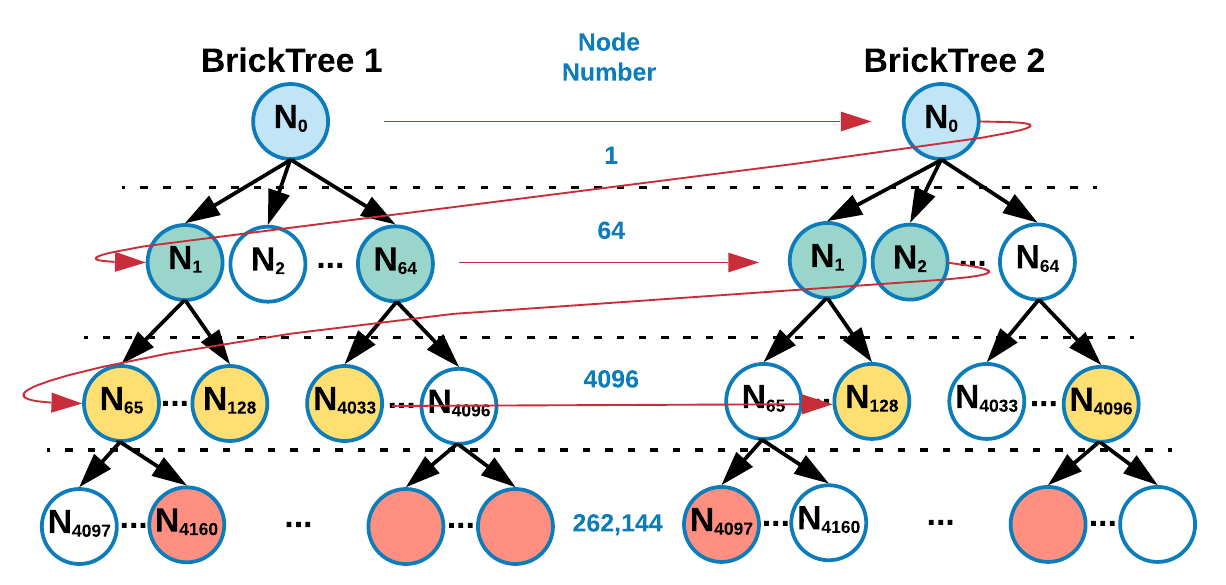
\includegraphics[width=0.5\textwidth]{LoadByLevel}
    \caption{\label{fig:loadbylevel}An illustration of streaming the valuebrick by level. Colored nodes are requested in current time. The red arrow indicates the loading sequence.}
    %\vspace{-1em}
\end{figure}

\begin{figure*}[t]
    \centering
    \begin{subfigure}[b]{0.85\columnwidth}
        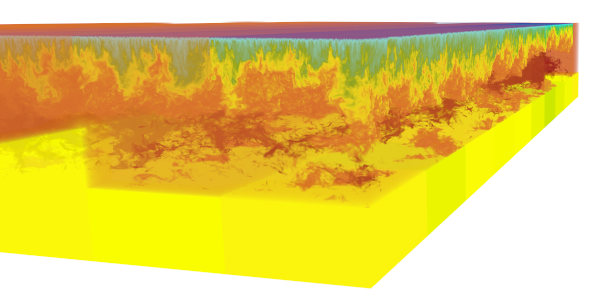
\includegraphics[width=\textwidth]{streambytree}
        \vspace{-2em}
        \caption{Stream by bricktree}
        \label{fig:streambytree}
    \end{subfigure}
    \begin{subfigure}[b]{0.85\columnwidth}
        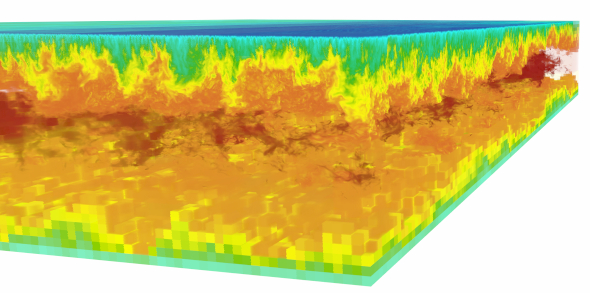
\includegraphics[width=\textwidth]{streambybrick}
        \vspace{-2em}
        \caption{Stream by valuebrick}
        \label{fig:streambybrick}
    \end{subfigure}
    \begin{subfigure}[b]{0.85\columnwidth}
        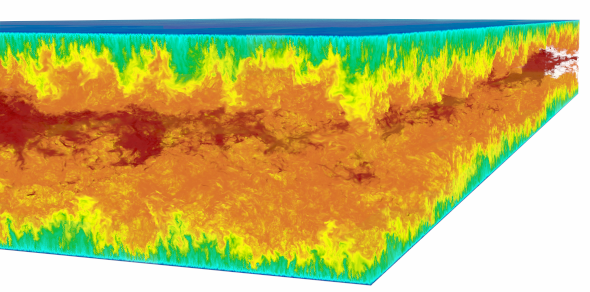
\includegraphics[width=\textwidth]{streambylevel}
        \vspace{-2em}
        \caption{Stream by tree level}
        \label{fig:streambylevel}
    \end{subfigure}
    \begin{subfigure}[b]{0.85\columnwidth}
        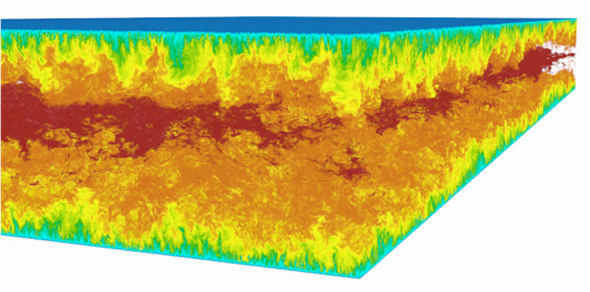
\includegraphics[width=\textwidth]{gound_truth}
        \vspace{-2em}
        \caption{Ground truth}
        \label{fig:streambylevel}
    \end{subfigure}
	\caption{\label{fig:streamstrategy}%
	A comparison of rendering image of the DNS dataset with three valuebrick loading strategies at frame 100. Stream by level shows more detail and smoother data refinement.}
	\vspace{-0.5em}
\end{figure*}


%-------------------------------------------------------------------------
\section{Ray-Guided Progressive Rendering}
The long waiting times of loading data from disk significantly
influence the user experience in an interactive visualization. 
In this section, we describe the solution to reducing IO latency with data streaming and progressive rendering. 
% we will discuss how we progressively stream and render the bricks
% represented by the bricktree forest.
Data streaming and rendering are decoupled in
our visualization pipeline. If requested data is not yet in memory, the renderer uses 
the average value stored in the (already loaded) parent node
and requests the missing brick from a data loading thread. Consequently,
the visualization process can be launched very quickly without waiting for the large
data to first be loaded into the memory. In addition, rendering performance remains stable 
when the camera position is updated. 


%----------------------------------
\subsection{Valuebrick Streaming}
So far, we have illustrated how we sample and traverse the bricktree assuming that all
multiresolution bricks are in memory, which works well on small- or moderate-size datasets. 
For large datasets, however, IO bottlenecks and memory size limit performance and rendering
quality. In particular, IO latency for loading the dataset into memory before
rendering becomes prohibitive when visualizing large data. Loading a
terascale dataset into memory on a contemporary workstation might take hours, even with a parallel IO
library such as PIDX. Furthermore, the memory might not be adequate to load all bricks. 


To solve this problem, we employ ray-guided progressive rendering and stream bricks
on demand. Although the idea behind this approach is similar to GigaVoxel\cite{crassin2009gigavoxels}
and to Hadwiger's work \cite{hadwiger2012interactive}, our implementation on multi-core CPUs
is more straightforward, and it avoids CPU-GPU communications and the complex data structures
needed to store the rendering context. As mentioned in~\Cref{sec:bricktree_layout},
each bricktree stores a linear array of valuebricks. All we need to do is maintain a
status for each valuebrick and update it correctly according to the rendering context.
In our solution, the \textit{isrequested} and \textit{isloaded} flags are
used to identify the current status of a valuebrick. In our sample function, 
the \textit{isrequested} flag of a valuebrick is set when we need to load the valuebrick
into memory, which allows us to implement a visibility-based solution that requests only
data that is inside the view frustum. 


%---------------------
\subsubsection{Progressive Sampling}
The sample function needs to be able to handle the equivalent of a cache miss -- the case
when a valuebrick is needed but not in the memory -- to generate a correct image.
One simple and synchronous approach mentioned in \cite{crassin2009gigavoxels} is to
load the missing valuebrick immediately and for volume integration to stop until 
the valuebrick is loaded. 
% The implementation in the GigaVoxel paper requires costly
% CPU-GPU communication, as well as an update of a CPU-hosted backing structure.
% Although our implementation does not involve a GPU, 
This approach is unacceptable for interactive visualization when many valuebricks are missing 
due to the prohibitive IO latency incurred by valuebrick loads. Given that the inner node
in the bricktree stores the average values of its child nodes, we adopted an
asynchronous approach for volume integration. We use the average value as an
approximation for the current sample point when we request the valuebrick and
refine the output image when the valuebrick is loaded in separate threads. 
\Cref{alg:sample_and_stream} depicts the pseudo-code of this process. 


%---------------------
\subsubsection{Valuebrick Loading Strategy}
In this work, multi-threading is employed to decouple the data streaming and rendering. 
We create independent threads that are responsible for determining the streaming sequence
and loading the requested valuebrick from the file system. These threads are able to access
the valuebrick buffer and update the \textit{isloaded} status when a valuebrick is loaded. 
Coordinated with the progressive sampling, an interactive and smooth visualization is achieved.

Although we achieve a stable framerate by decoupling the data streaming and rendering, the 
valuebrick loading sequence impacts the qualitative performance of our 
progressive refinement strategy. Given the layout of our bricktree, three choices are considered.

Recall from \Cref{sec:bricktree_layout} that the volume is encoded as a bricktree ``forest''. 
Hence, the naive approach is to map the whole bricktree into memory if a valuebrick in the
respective bricktree is requested. We refer to this approach as ``streaming by bricktree''. 
This approach is easy to implement but not efficient, because bricktrees tend to be large, 
and because many unrequested valuebricks will be loaded. 



A finer-granularity approach is to ``stream by valuebrick'' rather than by bricktree. For each
bricktree, the streaming threads will filter and load the requested valuebricks. 
This approach yields better performance than the first approach, since loading a valuebrick
is much cheaper than loading a bricktree. Visually, the user will notice a smoother and finer grained refinement (as shown in \Cref{fig:streambybrick}).
However, for the first few frames, when a large number of valuebricks are missing, performance is lackluster, since many valuebricks will be requested at once by the ray sample function.
In the worst case, we need to load almost all valuebricks
in the current bricktree before moving to the next bricktree, which results in a slight performance improvement over the first approach.



Generally, the data exploration process is ``overview first, zoom and filter, then detail-on-demand''
\cite{ferster2012interactive,wang2018association}. 
Following this mantra, 
the ideal approach is to update the data resolution progressively. 
In this work, we adopt an approach similar
to level-order tree traversal and load the requested valuebricks by level. \Cref{fig:loadbylevel}
illustrates this approach. Given a user-defined view frustum, the streaming thread
selects the requested valuebricks (colored) by level and pushes them into a queue to load. Due to
the large branching factor ($N^3$) of our hierarchical structure, only a small portion of the
nodes are inner nodes. For example, in \Cref{fig:loadbylevel}, using $4^3$ bricks to encode a
$512^3$ volume, only $1.6\%$ of the nodes are inner nodes. Consequently, loading the inner node levels
takes relatively little time, and we can achieve smooth visual refinement of our data. 
\Cref{fig:streamstrategy} compares visual refinement using different streaming strategies.




Another factor that improves progressive refinement performance is valuebrick load speed,
although this is highly dependent on IO throughput. Due to the design of the bricktree ``forest'', 
the levels of the bricktree can be loaded in parallel since each process is independent.
For example, we can load level 2 of tree 1 and tree 2 in parallel using $tbb::tasking\_parallel$. 
Compared to serial streaming, we observe that parallel streaming significantly improves performance. 


%----------------------------------
\subsection{Early Tree Traversal Termination}
So far, we have discussed a ray-guided visibility culling approach that allows our renderer
to load only the visible portion of the volume. The idea is, for a given viewport, that only part of the data
contributes to the final image. Similar ideas can be applied to improve 
rendering performance. In particular, under the right conditions, bricktree traversal
can be stopped at an inner node that reaches the appropriate level-of-detail (LOD). 

%--------------------- likely to use a phrase like "camera position" or even "view position". In this sentence, I changed "viewpoint" to "view frustum" because the blocks that get loaded does not only depend on the camera position, it also depends on the camera paramete likely to use a phrase like "camera position" or even "view position". In this sentence, I changed "viewpoint" to "view frustum" because the blocks that get loaded does not only depend on the camera position, it also depends on the camera paramete likely to use a phrase like "camera position" or even "view position". In this sentence, I changed "viewpoint" to "view frustum" because the blocks that get loaded does not only depend on the camera position, it also depends on the camera paramete likely to use a phrase like "camera position" or even "view position". In this sentence, I changed "viewpoint" to "view frustum" because the blocks that get loaded does not only depend on the camera position, it also depends on the camera paramete
\subsubsection{Level-of-Detail Control}
Some primitives are smaller than the output device pixels when rendering a
large dataset at low magnification\cite{rusinkiewicz2000qsplat}. Generally, in this case,
it is hard to tell the visual difference in the interactive rendering if we use higher resolution data. 
One general-purpose approach to 
reduce rendering time is to store data at a discrete level of detail and select a lower resolution LOD with primitives that more closely matches the display resolution. 

In this work, it is easy to apply LOD-based ideas since an inner node can be interpreted as
a coarser representation of its descendants. During traversal, we calculate the projected
screen space area of a valuebrick and stop the traversal if the area is smaller than a 
user-defined threshold. To simplify computation, we use a sphere as an approximation of a cubic
valuebrick. By setting the threshold to one pixel, we achieve a 2.5x speed-up when we 
zoom out and view the DNS dataset at low magnification. 


%---------------------
\subsubsection{Culling with Transfer Function}
We can stop the traversal when the valuebrick does not contribute to the 
final image given the current transfer function. In general, the performance of interactive visualization
depends on the user-defined transfer function.
For example, the framerate drops to 2-3 fps if we make the interior of the DNS volume transparent and keep the
top and bottom boundaries opaque, because rays terminate much later
when most of the volume is transparent. Furthermore, tree traversal is still performed on each
sample even when its corresponding valuebrick is transparent. Taking advantage of the value
range stored in each node, this can easily be avoided in our implementation. The callback
function \textit{getMaxOpacityInRange(cellRange)} allows us to look up the brick's maximum
opacity based on the current transfer function.
If the maximum opacity equals 0, the tree traversal stops at the 
current valuebrick and skips the descendants. Although the speed-up of this optimization
depends on the data and transfer function, we achieve an average 2x speed-up for
the DNS dataset with a transparent interior.



%-------------------------------------------------------------------------
\section{Results}
In this section, we evaluate four key aspects of our system: 1) the performance of the existing OSPRay
volume renderer and our bricktree module; 2) the performance of the bricktree with different brick sizes;
3) data compression using the bricktree; 4) the performance of bricktree generation. Unless otherwise noted,
benchmarks were performed on a quad-socket workstation (FSM) with four Xeon E7-8890 v3 CPUs, with a total
of 72 physical cores at 2.5 Ghz, along with 3 TB RAM. In the benchmark, volumes were rendered to a
$1024 \times 768$ framebuffer, and the rendering performance was measured by calculating the average
framerate over 100 frames.   


We tested our renderer with four datasets with sizes ranging from small (e.g., magnetic 
reconnection volume\cite{guo2014formation}), to medium (e.g., the Richtmyer-Meshkov instability simulation
\cite{cohen2002three} and cardiac volume\cite{scivisdata}) to extremely large (e.g., the DNS dataset \cite{moser1999direct}).
\begin{itemize}
\item The magnetic volume, produced from kinetic simulations, is a $512^3$ float-precision dataset
(size: 512 MB) that represents magnetic reconnection in relativistic plasmas. 
\item The Richtmyer-Meshkov instability (RMI) is a simulation of carbon hexafluoride being pushed up through a wire mesh, with a resolution of $2048 \times 2048 \times 1920$ and data type of uint8 (size: 8.1 GB). It is a popular dataset and is also used in \cite{fogal2013analysis, wu2018visit, knoll2006interactive}. 
\item The cardiac volumes were obtained by way of computed tomography (CT) imaging on excised,
postmortem porcine hearts. The resolution of the data is $2048 \times 2048 \times 2612$. With a data
type of int16, the size of the data goes up to 21 GB. 
%  Alginate curing agents were injected into ventricles to provide rigidity and radiopaque agents were injected into the coronary arteries to distinguish microvasculature from the rest of the tissue
\item The DNS, produced by the Institute for Computational Engineering and Science (ICES) at the University
of Texas-Austin is a single $10240 \times 7680 \times 1536$ double precision volume (size: 900 GB) from a turbulent flow simulation. 
\end{itemize}

\begin{figure}[h]
    \centering
    \begin{subfigure}[b]{0.9\columnwidth}
        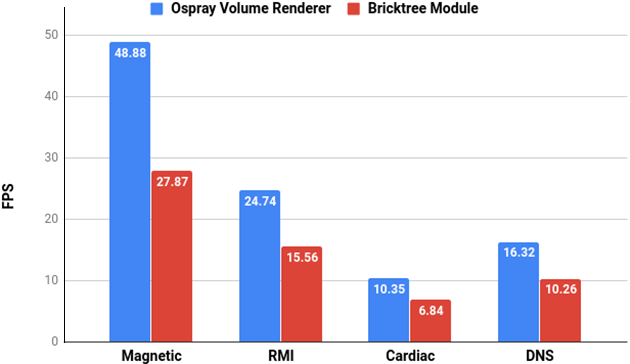
\includegraphics[width=\textwidth]{exp_ospray_bricktree_1}
        \vspace{-2em}
        \caption{Overall performance}
        \label{fig:exp_ospray_bricktree_framerate}
    \end{subfigure}
    \begin{subfigure}[b]{0.9\columnwidth}
        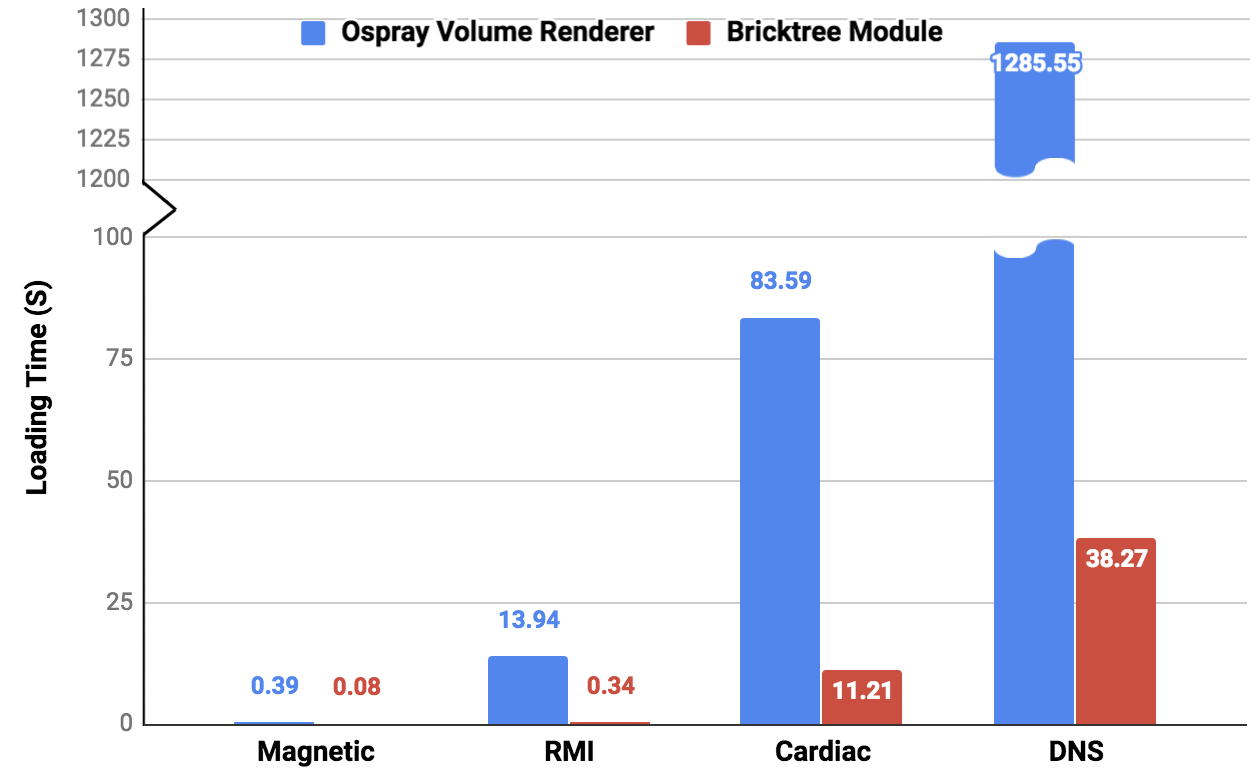
\includegraphics[width=\textwidth]{exp_ospray_bricktree_2}
        \vspace{-2em}
        \caption{Waiting time before rendering the first frame}
        \label{fig:exp_ospray_bricktree_waitingtime}
    \end{subfigure}
	\caption{\label{fig:exp_ospray_bricktree}%
	A comparison of overall performance and loading time between existing OSPRay volume renderer and our bricktree module. The evaluation was run on bricktree with a brick size of 4.}
	\vspace{-0.5em}
\end{figure}

%----------------------------------
\subsection{Existing OSPRay Renderer vs. Bricktree Module}
Although the existing OSPRay volume renderer provides limited support for rendering large 
volumes on CPU, it can suffer from prohibitive IO latency because all 
the data must be loaded into memory before the first frame can be rendered.

\feng{
\Cref{fig:exp_ospray_bricktree} shows the trade-off between overall performance
and loading time when using the OSPRay volume renderer and bricktree module.
It is shown that the overall performance of the bricktree module is around $35\%$
lower compared to the existing OSPRay volume renderer, since we need to traverse
the hierarchy to query the data value in the bricktree module. This is in contrast
to the data query in existing OSPRay module with simple math calculations.
Although we suffer a bit performane loss, \Cref{fig:exp_ospray_bricktree_framerate}
indicates that the bricktree module still allows the renderer to run at interactive rates. 
}

\feng{
On the other hand, we measured the waiting time before the renderer yields the first frame
(\Cref{fig:exp_ospray_bricktree_waitingtime}). The bricktree module achieves much better 
performance than the existing OSPRay volume renderer since it needs to
load only metadata prior to rendering. The loading time of both renderers increases with
data size. However, the bricktree module slows down much less. For instance, without
the bricktree module, users must wait more than 20 minutes on FSM before being able
to see a ``bird's eye view'' of the DNS dataset. By contrast, with the bricktree module,
the DNS dataset loads in under 40 seconds. Therefore, we believe that the bricktree 
module is a better choice for rendering large datasets, whereas the existing OSPRay
volume renderer works better for small- to moderate-size datasets. 
}



%----------------------------------
\subsection{Choice of Brick Size}
\label{sec:exp_bricksize}

A volume renderer's domain decomposition method can have a large impact on the 
performance of the rendering pipeline\cite{fogal2013analysis}. Our design and 
implementation allow the user to easily set a custom brick size. 
We performed a set of experiments to discover how the brick size affects the
tree generation time, tree size, loading time, streaming performance and overall
framerate. Two datasets were tested: RMI (8.1 GB, int8), which is a sparse dataset, and
DNS(450 GB, float), which is a very dense dataset.

\begin{table}[h!]
	\centering
	\begin{tabularx}{\linewidth}{l*{4}{r}}
		\toprule  
		\textbf{RMI / Brick Size}   & \textbf{2} & \textbf{4} & \textbf{8} & \textbf{16}  \\
		\hline
		Tree Build (min) & 1.61 & 1.49 & 1.34 & 1.96  \\
        Tree Size (GB) & 7.80 & 5.90 & 7.10 & 9.60  \\
        Loading Time (s) & 1.48 & 0.34 & 0.15 & 0.56  \\
        Stream Performance (s) & 0.21 & 0.13 & 0.11 & 0.08  \\
        Framerate (fps) & 10.56 & 18.56 & 10.75 & 7.78  \\
		\bottomrule
	\end{tabularx}
    \begin{tabularx}{\linewidth}{l*{4}{r}}
		\toprule  
		\textbf{DNS / Brick Size}   & \textbf{2} & \textbf{4} & \textbf{8} & \textbf{16}  \\
		\hline
		Tree Build (min) & 177.22 & 92.93 & 86.66 & 80.25  \\
        Tree Size (GB) & 772 & 486 & 455 & 451  \\
        Loading Time (s) & 92.26 & 38.27 & 9.3 & 7.67  \\
        Stream Performance (s) & 0.18 & 0.16 & 0.13 & 0.08  \\
        Framerate (fps) & 15.36 & 18.38 & 36.63 & 45.62  \\
		\bottomrule
	\end{tabularx}
	\caption{An evaluation of tree build time, tree size, loading time, stream performance (s/1000 valuebricks) and overall performance with different brick sizes on a sparse dataset (RMI) and a dense dataset (DNS). The evaluataion was run on FSM. The tree build process was executed in parallel with eight processors.}
	%\vspace{-1em}
	\label{table:brick_size}
\end{table}

\Cref{table:brick_size} shows rendering performance with different brick sizes.
As we know, the smaller valuebrick size is more likely to be uniform in value 
\cite{fogal2013analysis}. In our unbalanced bricktree, a valuebrick that contains
uniform values will not be further decomposed and stored by adopting a lossless 
fashion (mentioned in \Cref{sec:hierarchy_generation}) and setting the threshold 
to the default value (0). Under this consideration, domain decomposition with a 
small brick size is more likely to yield a bricktree with fewer valuebricks. 
Therefore, a small brick size is more suitable for storage and probably fast traversal. 

However, the results in \Cref{table:brick_size} indicate a slightly
different conclusion for different datasets. For a sparse dataset (e.g., RMI),
a brick size of 4 produces a smaller tree and performs better than a brick size of 8 or 16. A brick size of 2 hampers performance and tree size, possibly due to an increased number of inner nodes resulting from greater tree depth. 

\begin{figure}[t]
    \centering
    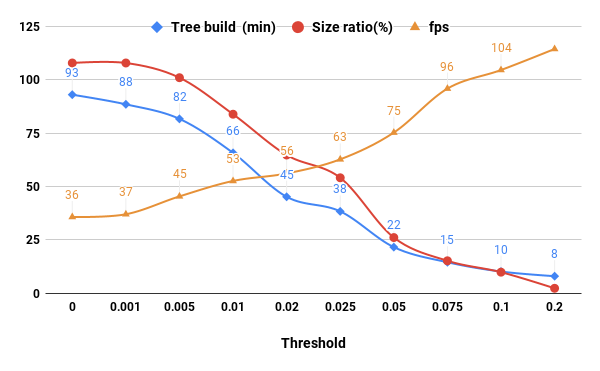
\includegraphics[width=\columnwidth]{exp_threshold}
    \vspace{-2em}
	\caption{\label{fig:exp_threshold}%
	A comparison of tree build time, size ratio (tree size / volume size) and overall performance with different thresholds on the DNS dataset.}
	\vspace{-0.5em}
\end{figure}


For a dense dataset (e.g., DNS), where values vary in almost all cells,
the output bricktree is most likely a balanced tree. Hence, we found that
a smaller brick size results in a larger tree size and longer construction time.
From the perspective of streaming performance, a large brick size is preferable 
for disk performance. For instance, the size of a valuebrick with a
brick size 16 is 4~KB, which equals the size of a single memory page on FSM. 
Therefore, a brick size of 16 gives more a friendly memory access pattern. 
We observed that the streaming thread will influence rendering performance
when many valuebricks are requested. For performance reasons, we believe that a 
large valuebrick size is more appropriate for visualizing dense datasets. 
\Cref{table:brick_size} demonstrates that, for the DNS dataset, rendering
performance is the best when a brick size of 16 is used. 

\begin{figure*}[t]
    \centering
    \includegraphics[width=\textwidth]{exp_threshold_2_b}
	\caption{\label{fig:exp_threshold_2}%
	A comparison of the output image rendered with four thresholds on the magnetic dataset (512~MB).
	With an appropriate threshold, such as 0.05, we achieve significant performance improvement and produce a final image that is slightly different with ground truth (thres: 0).
% 	Qualitatively, only a slight difference can be discerned in the images.
	}
	%\vspace{-0.5em}
\end{figure*}

\subsection{Bricktree Compression}
In ~\Cref{sec:hierarchy_generation}, we described how a threshold could be specified 
in order to collapse a specific input region of volume during the hierarchy generation.
By using the default value 0, we produced a lossless hierarchical representation of
the volume. \Cref{sec:exp_bricksize} indicates that this lossless compression
is satisfactory for a sparse dataset since regions with uniform values
are collapsed. However, a lossy representation is generated if the threshold is
set to a positive value. ~\Cref{fig:exp_threshold} displays bricktree build time,
the ratio of the bricktree's size to raw volume and the rendering performance given different 
thresholds over the DNS dataset. The build time and tree size drop dramatically when 
the threshold is increased, and the rendering performance improves significantly. 
A detailed quantitative analysis of the accuracy of the output image over different 
thresholds is beyond the scope of this paper.
However, \Cref{fig:exp_threshold_2}
depicts the output image of the magnetic dataset rendered with four thresholds. Aside from the performance improvement, 
we observe that only a slight difference can be discerned in the final images if we select an appropriate threshed (e.g., 0.05) for the magnetic dataset.
On the other hand, artifacts emerge when the data is visualized with a large threshold (e.g., 0.3).
% Qualitatively, 
% there is only a slight difference in the output images.

\begin{figure}[h]
    \centering
    \begin{subfigure}[b]{0.32\columnwidth}
        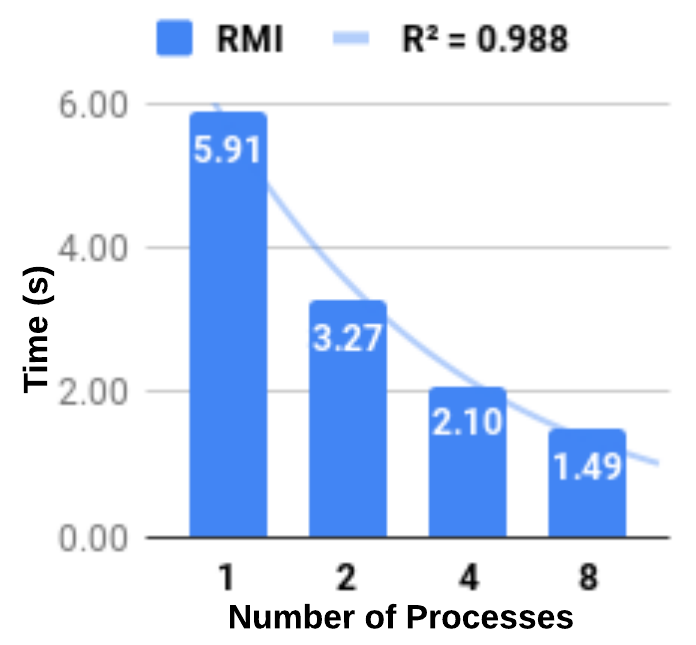
\includegraphics[width=\textwidth]{exp_buildtime_1}
        \vspace{-1.5em}
        \caption{RMI}
        \label{fig:exp_buildtime_1}
    \end{subfigure}
    \begin{subfigure}[b]{0.32\columnwidth}
        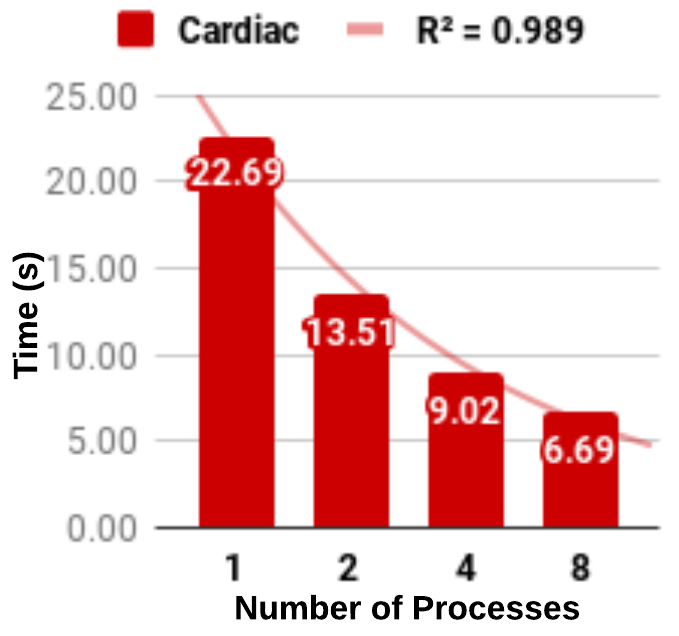
\includegraphics[width=\textwidth]{exp_buildtime_2}
        \vspace{-1.5em}
        \caption{Cardiac}
        \label{fig:exp_buildtime_2}
    \end{subfigure}
    \begin{subfigure}[b]{0.32\columnwidth}
        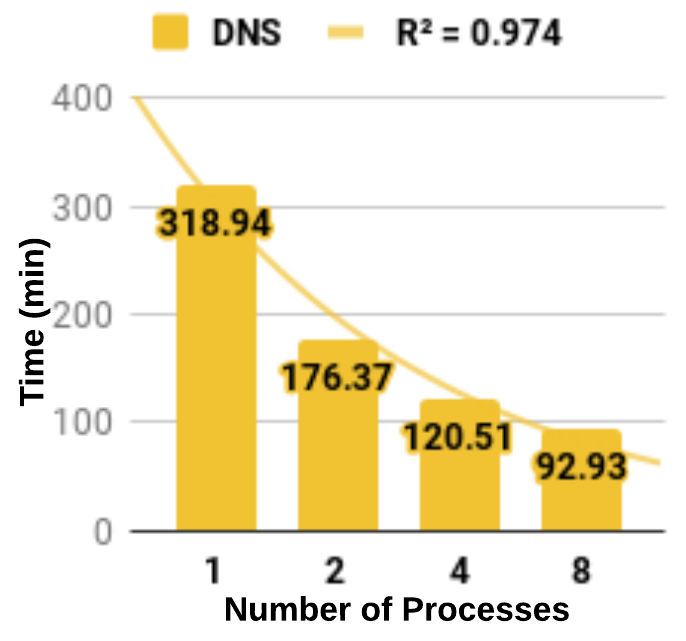
\includegraphics[width=\textwidth]{exp_buildtime_3}
        \vspace{-1.5em}
        \caption{DNS}
        \label{fig:exp_buildtime_3}
    \end{subfigure}
   
	\caption{\label{fig:exp_buildtime}%
	Tree build time by running the \textit{ospRawToBrick} tool with different numbers of processes on three datasets. The brick size of the bricktree is set to 4 in this evaluation.}
	\vspace{-0.5em}
\end{figure}

\subsection{Bricktree Generation}

Although hierarchy generation performance has drawn less attention than rendering
performance, it is a significant bottleneck in real-world usage\cite{fogal2013analysis}. 
In this section, we evaluate the performance of the ``\textit{ospRawToBrick}'' tool. 
Tree generation time, which benefits from the parallel build processes, drops
dramatically by running multiple jobs simultaneously. \Cref{fig:exp_buildtime} shows
 hierarchy generation time with three datasets. For the RMI dataset, \cite{fogal2013analysis} claims that the generation time of their hierarchy structure takes
about 13 minutes in the best case. However, with our solution, it only takes 1.49 seconds using eight processes. 



\section{Conclusion}
In this paper, we have presented a solution for interactive visualization of 
large volumes on multi-core CPU architectures. Our method is based on  
hierarchical representation and ray-guided progressive rendering that 
allows the user to view and explore hundreds of gigabytes of data without
spending minutes or even hours waiting for data to load. 
Our solution is a significant improvement compared to the existing OSPRay volume renderer,
which usually takes minutes or hours to load the data prior to rendering the first frame. 
Inspired by many recent renderers, we present a hierarchical data structure
-- a bricktree -- with a large branching factor and relatively low overhead. We have
also evaluated and discussed the tradeoffs of the different 
parameters. Based on our experimental results, we conclude that sparse datasets 
are best used with small brick sizes (e.g., 4), and dense datasets are best used with 
large brick sizes (e.g., 16). 

Our data structure naturally facilitates compression. Using the bricktree to create an easy-to-implement lossless compression scheme, we reduced the size of the RMI dataset from 8.1~GB to 5.9~GB with a brick size of 4 
(\Cref{table:brick_size}). Furthermore, this scheme can easily be extended to support lossy compression.

Finally, we implemented our solution as a module for the OSPRay ray tracing framework. Since OSPray is already interfaced with tools like ParaView and VisIt, users should have no difficulty putting our results into production.

%Our OSPRay module can also be leveraged by existing work integrating OSPRay into ParaView and VTK, to provide similar results to production visualization users. 

In the future, we hope to further investigate data compression.  
For instance, valuebricks are natural candidates for float-point data compression using ZFP
\cite{lindstrom2014fixed}.
Furthermore, a detailed quantitative analysis of how the lossy compression
threshold affects final image quality should be performed. 
Eventually, we would like to integrate the bricktree module into
general-purpose visualization frameworks. 



%-------------------------------------------------------------------------

%% if specified like this the section will be committed in review mode
\acknowledgments{
The authors wish to thank A, B, and C. This work was supported in part by
a grant from XYZ.}

%\bibliographystyle{abbrv}
\bibliographystyle{abbrv-doi}
%\bibliographystyle{abbrv-doi-narrow}
%\bibliographystyle{abbrv-doi-hyperref}
%\bibliographystyle{abbrv-doi-hyperref-narrow}

\bibliography{bricktree}

%-------------------------------------------------------------------------
\end{document}
